\documentclass[a4paper,12pt]{article}

\usepackage{graphicx}
\usepackage{hyperref}
\usepackage[italian]{babel}
\usepackage{parskip}
\usepackage{multicol}
\usepackage{verbatim}
\usepackage[a4paper,left=2cm,right=2cm,top=2.5cm,bottom=2.5cm]{geometry}
\usepackage{float}
\usepackage{setspace}
\usepackage{svg}
\usepackage{amsmath}
\usepackage{wrapfig}

\setlength{\parskip}{1em}
\graphicspath{ {./images/} }
\hypersetup {
    colorlinks=true,
    linkcolor=black,
    urlcolor=blue,
    citecolor=blue,
    pdfborderstyle={/S/U/W 1},
    }
\pagenumbering{gobble}
    \begin{document}
    \begin{titlepage}
        \begin{center}
            \begin{minipage}{0.3\textwidth}
                
\includegraphics[width=\linewidth]{Logo_Universita.png}
            \end{minipage}

        \end{center}

        \begin{center}
            \noindent\rule{0.7\textwidth}{0.4pt}\\[0.5cm]
            \large\textbf{Università degli Studi di Padova}\\
            \large Corso di Laurea in Informatica\\
            \small A. A. 2025/26
        \end{center}

        \vspace{1,5cm}    

    \begin{center}
        \begin{minipage}{0.5\textwidth}
            \includesvg[width=\linewidth]{logo}
        \end{minipage}
    \end{center}

        \vspace{1,5cm}    
        \begin{center}
            {\Large \textbf{Relazione}\par}
            \vspace{0.6cm}
            {\Large Concorso Accattivante Accessibile\par}
            \vspace{0.3cm}
        \end{center}
        \vfill

        \centering
        \begin{tabular}{r|l}
            \textbf{Studenti} & Sofia De Blasi (referente) - 2111014 - \underline{\href{mailto:sofia.deblasi@studenti.unipd.it}{sofia.deblasi@studenti.unipd.it}}\\
             & Nicola Simionato - 2113190 - \underline{\href{mailto:nicola.simionato.5@studenti.unipd.it}{nicola.simionato.5@studenti.unipd.it}} \\
            & Nenad Radulovic - 2101059 - \underline{\href{mailto:nenad.radulovic@studenti.unipd.it}{nenad.radulovic@studenti.unipd.it}} \\
            & Giacomo Speggiorin - 2116438 - \underline{\href{mailto:giacomo.speggiorin@studenti.unipd.it}{giacomo.speggiorin@studenti.unipd.it}} \\
            & \\
            \textbf{Indirizzo del sito} & \underline{\url{https://caa.studenti.math.unipd.it/sdeblasi/}}\\
            & \\
            \textbf{Utente} & 
            \textbf{Username:} user, \textbf{Password:} user \\ 


        \end{tabular}

        \vfill

    \end{titlepage}  
    \newpage
\clearpage 
\pagenumbering{arabic}
\section{Introduzione}

Il progetto \emph{Student Space} è stato realizzato con l’obiettivo di dimostrare che un sito web 
può essere al tempo stesso accessibile, gradevole e funzionale, in linea con lo spirito del 
concorso \emph{Accattivante Accessibile}. La piattaforma raccoglie annunci utili alla vita 
universitaria (eventi, affitti, ripetizioni, esperimenti) e permette agli utenti di consultarli, 
filtrarli e pubblicarli in modo semplice e intuitivo.

Fin dalle prime fasi di progettazione, il lavoro è stato guidato dai principi delle WCAG~2.1 
livello~AA, adottando un approccio orientato alla fruibilità per tutte le 
categorie di utenti. Ogni scelta relativa a struttura, contenuti, interazioni e design è stata 
valutata in funzione della sua accessibilità, con particolare attenzione alla semantica HTML, 
alla navigazione da tastiera, alla gestione dei testi alternativi, ai contrasti cromatici e alla 
prevedibilità dei comportamenti dell’interfaccia.

L’obiettivo finale è stato quello di creare un sito che non richieda all’utente di adattarsi, ma 
che si adatti alle sue esigenze.

\section{Accessibilità}

\subsection{Strumenti di verifica}

Sono stati utilizzati diversi strumenti di verifica:
\begin{itemize}
    \item \textbf{NVDA}: per testare la gerarchia dei titoli, la lista dei link e dei punti di riferimento, la navigazione tramite landmark e l’annuncio dei messaggi di errore nei form, sia con JavaScript attivo che disattivato.
\end{itemize}

\begin{itemize}
    \item \textbf{Contrast Checker} (\underline{\url{https://contrastchecker.com/}}): per verificare il rispetto del rapporto di contrasto $\geq 4.5\!:\!1$.
    \item \textbf{Lighthouse, Silktide e strumenti di ispezione (F12)}: per valutazioni automatiche e test manuali su navigazione da tastiera, accessibilità dei link, dimensioni degli elementi cliccabili e altri criteri WCAG.
\end{itemize}

\subsection{Struttura semantica e navigazione}

Il codice HTML utilizza landmark semantici (\texttt{header}, \texttt{nav}, \texttt{main}, 
\texttt{aside}, \texttt{footer}), evitando tag puramente presentazionali e una gerarchia coerente di titoli (\texttt{h1-h4}), infatti: le card degli annunci (\texttt{cardTemplate.html}) utilizzano \texttt{<h3>} per i titoli, evitando coppie \texttt{<dt>}–\texttt{<dd>}.  
In tale modo la gerarchia semantica è preservata: \texttt{<h2>} identifica la sezione (es. “Ultimi inseriti”), mentre \texttt{<h3>} rappresenta ciascun annuncio. 

La navigazione è stata progettata per essere chiara e prevedibile:
\begin{itemize}
    \item breadcrumb con \texttt{aria-current};
    \item menu responsive accessibile da tastiera;
    \item caroselli non ciclici per evitare loop infiniti;
    \item link sempre descrittivi e mai generici.
\end{itemize}

\subsection{Immagini e testi alternativi}

Le immagini above-the-fold usano \texttt{loading="eager"}, tutte le altre \texttt{lazy}.  
Sono stati, poi, adottati formati ottimizzati (SVG per il logo, WebP per decorative, JPG per gli annunci) 
e dimensioni inferiori a 1~MB.

Nel form di pubblicazione l’utente deve scegliere se l’immagine è decorativa o descrittiva e in tal caso il testo alternativo è obbligatorio e limitato a 100 caratteri per garantire sintesi e usabilità con screen reader.  

Inoltre, le immagini degli annunci hanno dimensioni definite via HTML per migliorare il rendering.

\subsection{Form e messaggi di errore}

I form utilizzano \texttt{fieldset} e \texttt{legend}, con etichette sempre associate ai campi.  
La validazione è multilivello:
\begin{itemize}
    \item HTML5 (\texttt{required}, \texttt{min}, \texttt{max}, \texttt{step});
    \item JavaScript con messaggi \texttt{role="alert"} e gestione del focus;
    \item PHP con la stessa struttura semantica degli errori lato client.
\end{itemize}

Il focus viene portato automaticamente sul primo campo non valido, con selezione del contenuto 
alla prima comparsa dell’errore.

\subsection{Tipografia e leggibilità}
Per garantire una lettura chiara e accessibile sono stati scelti due font distinti:

\begin{itemize}
    \item \textbf{Web}: \emph{Noto Sans}, importato tramite Google Fonts.
    \item \textbf{Stampa}: \emph{Times New Roman}.
\end{itemize}

La scelta del font web è stata guidata da verifiche sulla leggibilità di caratteri critici (\texttt{qp, db, 0O, iI1l, rn, m}), sull’altezza della \emph{x} e  sull'apertura delle lettere \emph{c} e \emph{a}.  
Inizialmente era stato considerato \texttt{Inter}, poi sostituito da \texttt{Noto Sans} per una migliore distinzione di glifi come \texttt{ca} e \texttt{iI1l} (vedi Figure~\ref{fig:font1} e~\ref{fig:font2}).

\begin{figure}[h!]
    \centering
    \begin{minipage}{0.48\textwidth}
        \centering
        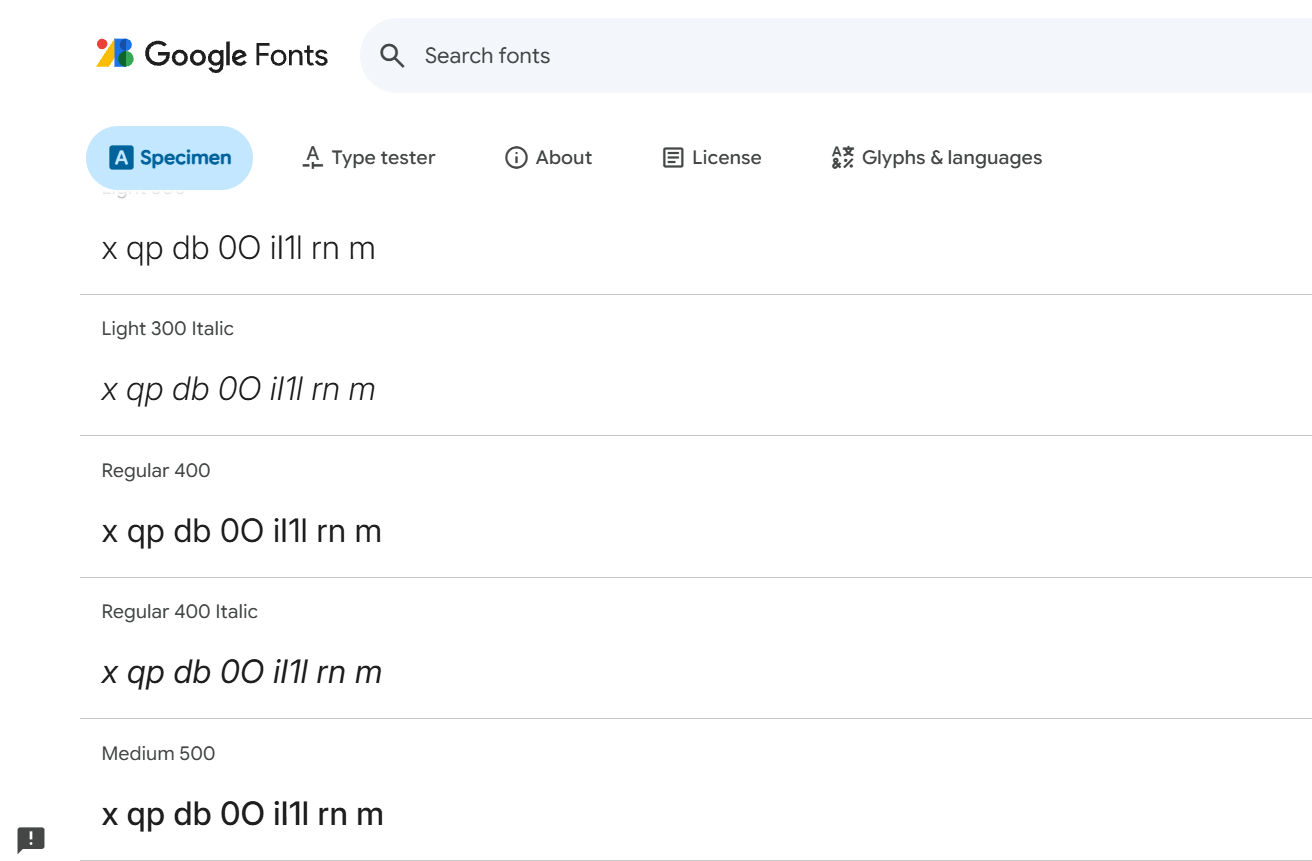
\includegraphics[width=0.7\textwidth]{inter.png}
        \caption{Font: Inter}
        \label{fig:font1}
    \end{minipage}
    \hfill
    \begin{minipage}{0.48\textwidth}
        \centering
        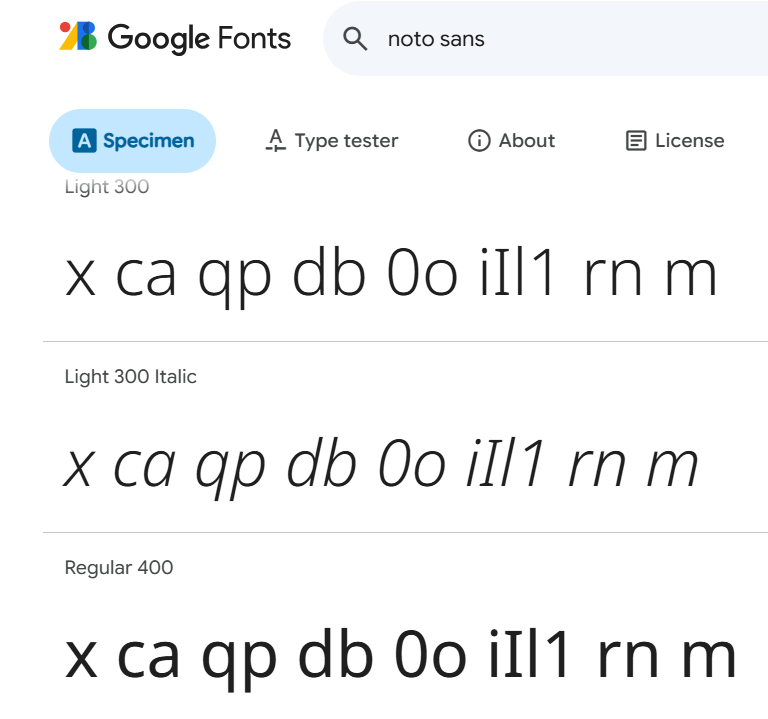
\includegraphics[width=0.7\textwidth]{noto.png}
        \caption{Font: Noto Sans}
        \label{fig:font2}
    \end{minipage}
\end{figure}

\paragraph{Leggibilità dei prezzi}
La funzione PHP \texttt{Tool::formatPrezzo()} formatta i valori numerici mostrando i decimali solo quando necessario (es. \texttt{20€} invece di \texttt{20.00€}), migliorando la leggibilità.

\subsection{Colori, contrasti e accessibilità mobile}

Sono stati adottati diversi accorgimenti per garantire una corretta percezione dei contenuti e la riconoscibilità degli elementi interattivi:

\paragraph{Link e Call To Action (CTA)}
    \begin{itemize}
        \item I link testuali sono sempre sottolineati.
        \item I link visitati/non visitati nella navbar e nelle card annunci differiscono per colore (contrasto 2.72 $\approx 3$) mentre nelle card di categoria il colore del \texttt{:visited} è associato al colore della categoria con contrasto $\geq 3$.
        \item I pulsanti CTA variano colore tra stato visitato e non visitato (in \texttt{background-color} e \texttt{color}).
    \end{itemize}
    (\href{https://caa.studenti.math.unipd.it/sdeblasi/relazione/sommario-contrasti.pdf}{\underline{Apri il Sommario dei Contrasti} }(PDF, 34 KB))


\paragraph{Accessibilità touch su mobile}
    \begin{itemize}
        \item Gli elementi cliccabili rispettano dimensioni minime di circa 44px × 44px.
        \item Il pannello laterale dei filtri utilizza un overlay e una gestione del focus accessibile \\(\texttt{toggleFiltriAccessibile()}).
        \item I pulsanti dei caroselli hanno opacità testata e leggibile (\texttt{rgba(22, 40, 110, 0.65)}).
    \end{itemize}

\section{Validazione, sicurezza e gestione degli errori}
\label{sviluppo:validazione}

\subsection{Errori lato client (JavaScript)}
La validazione lato client fornisce un feedback immediato e migliora l’esperienza d’uso, ed è attiva solo nei form che dichiarano l’attributo \texttt{data-validate}, così da non interferire con i form più semplici. All’avvio della pagina lo script controlla la presenza di eventuali errori generati dal server: se riguardano le immagini il focus viene portato sul primo \texttt{input file}, mentre per errori testuali viene selezionato il primo campo non valido; la selezione del contenuto e il trasferimento del focus avvengono solo alla prima comparsa dell’errore per evitare comportamenti troppo restrittivi e bloccanti.

La validazione avviene in tre momenti: al \texttt{blur} del campo, durante l’\texttt{input} (che rimuove messaggi e ripristina gli attributi ARIA) e al \texttt{submit}, quando tutti i campi vengono controllati e l’invio viene eventualmente bloccato. La funzione \texttt{validateField()} applica controlli specifici per i campi principali (nome, cognome, email, password, conferma password, città e consenso email), mentre campi come \texttt{file}, \texttt{alt} e \texttt{decorativa} sono esclusi dalla validazione client-side. Gli errori vengono mostrati tramite un contenitore dedicato con elementi dotati di \texttt{role="alert"} e con l’applicazione dinamica di \texttt{aria-invalid} e \texttt{aria-describedby}; la funzione \texttt{removeError()} rimuove automaticamente contenitore e attributi non più necessari.

\subsection{Errori lato server (PHP)}

La validazione lato server garantisce un comportamento corretto anche senza JavaScript, mantenendo coerenza con la validazione client-side. Gli errori riguardano campi generici, immagini (dimensione, formato, testo alternativo) e credenziali di accesso, e vengono restituiti con la stessa struttura semantica dei messaggi lato client, sempre tramite elementi con \texttt{role="alert"}. Anche qui vengono applicati dinamicamente \texttt{aria-invalid} e \texttt{aria-describedby}, e il focus viene portato sul primo campo non valido o sul primo \texttt{input file} in caso di errori relativi alle immagini.

Per le immagini vengono controllati dimensione (1 MB), formati consentiti (JPG lato form, JPG/PNG/WEBP lato server) e obbligatorietà del testo alternativo quando l’immagine non è decorativa. Nel login, eventuali errori vengono gestiti tramite messaggi contestuali e tramite il sistema \texttt{redirectMessage}, che informa l’utente del motivo del reindirizzamento.

Per la sicurezza degli input viene utilizzata la funzione \texttt{strip\_tags()}, che rimuove i tag HTML e PHP mantenendo però il testo interno. Questa scelta evita l’inserimento di markup indesiderato senza introdurre messaggi di errore aggiuntivi, mantenendo coerenza tra i vari form: il contenuto viene preservato quando l’utente usa markup con intento semantico, mentre un uso massiccio o sospetto di tag viene neutralizzato assumendo che possa trattarsi di un tentativo malevolo.

\section{Testing}
\subsection{Navigazione da tastiera}

È stato controllato l’ordine di tabulazione, la gestione del focus nei pannelli a scomparsa 
(es. filtri) e l’attivabilità di tutti gli elementi interattivi tramite tastiera.  
Particolare attenzione è stata dedicata all’\texttt{aside} dei filtri, che utilizza overlay e 
focus trapping.

\subsection{Test con utenti reali}
Per garantire che il comportamento del sito fosse chiaro, prevedibile e accessibile, abbiamo svolto una serie di test con utenti esterni al gruppo di sviluppo. Essendo noi i creatori del sistema, avremmo potuto non accorgerci di elementi poco intuitivi; per questo abbiamo coinvolto persone con profili diversi: studenti di varie facoltà, ex studenti, genitori e una persona con mobilità limitata che utilizza una sola mano. Questo ci ha permesso di osservare l’interazione da prospettive differenti e di verificare che l’esperienza d’uso rimanesse comprensibile e coerente per utenti con esigenze e competenze eterogenee.

\end{document}
